\chapter{Test Plan} \label{Chp:TestPlan}

There are two aspects to software testing:

\begin{itemize}
\item \textbf{Validation} to verify that the software gives the correct/desired results: after implementation of new features, and major bug fixes.
This is typically a manual process.
\item \textbf{Regression} to verify that the software continues to give the same results after an update (except for the changed, removed, or added functionality, of course).
This repetitive work can be automated.
\end{itemize}


\section{Validation}

For the verification of \dfastmi 2.0 four sets of input files for the Nederrijn River were used:

\begin{enumerate}
\item One set of input files exported from WAQUA via WAQVIEW.
\item One set of WAQUA files converted using \file{sim2ugrid.m} to \dflowfm like netCDF files.
\item One set of \dflowfm simulations using the same curvilinear mesh as was used in WAQUA.
\item One set of \dflowfm simulations using a new unstructured mesh.
\end{enumerate}

For the verification of \dfastmi 3.0 applications on Nederrijn, Pannerdensch Kanaal and Meuse have been used.
The argumentation is reported separately (in a `Validation report').


\section{Regression}

Regression testing is applied at different levels:

\begin{itemize}
\item \textbf{Unit} tests are designed to test specific functional elements.
It needs to strike a balance between detailed testing of each and every program construct (which is implementation specific and hence hinders easy restructuring of old code) and higher level tests that test too much functionality at once such that you still don't know where a problem is when it fails.

\item \textbf{Integration} tests are designed to test a common workflow across two or more functional elements.
The main routines \keyw{batch\_mode} and \keyw{interactive\_mode} are tested at this level via regression tests.

\item \textbf{System} tests are designed to test a full workflow across all functional elements.
Depending on the testing phase (source code, or binary, see below) the system tests execute the code starting from the command line parsing in \keyw{\_\_main\_\_.py} (binary testing) or viacalls to the \keyw{run} function in the \keyw{cmd} module (source code testing).

\item \textbf{Acceptance} tests are designed to test that the system works for specific use cases (the acceptance models).
\end{itemize}

The regression testing is applied two times:

\begin{itemize}
\item \textbf{Source code} The first regression test bench runs from the source code within Python.
This is the only point in time to efficiently run unit tests and integration tests.
At this point in time we also run a number of basic system tests.
This test bench currently contains 456 tests.
For a summary of the tests, see \autoref{Tab:SourceRegressionTests}.
The system tests in this phase call the \keyw{run} function in the \keyw{cmd} module.

\item \textbf{Binary} The second regression test bench tests the binary.
This is limited to system and acceptance tests only.
This test bench currently contains 10 tests.
For a summary of the tests, see \autoref{Tab:DistRegressionTests}.
All tests in this phase enter the code via the command line parsing implemented in \keyw{\_\_main\_\_.py}.
Several of these tests are also executed in during the source code testing phase.
\end{itemize}

For both test benches we use the pytest framework.
In the first case, that's a natural choice given the integration within the Python environment.
In the second case, other tools could have been used, but we use the same tool for consistency.
In this case, the binaries are started as an external process from within the Python tests providing as necessary streamed input and capturing the output.

\begin{longtable}{l|l}
\caption{Overview of testing within Python}\label{Tab:SourceRegressionTests} \\
File & Number of tests \\ \hline
\endfirsthead
\multicolumn{2}{l}{\textsl{(continued from previous page)}} \\
File & Number of tests \\ \hline
\endhead
\hline \multicolumn{2}{r}{\textsl{(continued on next page)}} \\
\endfoot
\hline
\endlastfoot

tests/test\_cli.py & 2 \\
tests/batch/Test\_AnalyserWaqua.py & 24 \\
tests/batch/Test\_Configuration\_Initializer.py & 6 \\
tests/batch/Test\_FileNameRetrieverFactory.py & 12 \\
tests/batch/Test\_FileNameRetriever\_legacy.py & 3 \\
tests/batch/Test\_FileNameRetriever\_unsupported.py & 1 \\
tests/batch/Test\_ReporterWaqua.py & 1 \\
tests/batch/Test\_configuration\_checker\_factory.py & 4 \\
tests/batch/Test\_configuration\_checker\_legacy.py & 12 \\
tests/batch/test\_AnalyserAndReporterDflowfm.py & 36 \\
tests/batch/test\_AnalyserDflowfm.py & 18 \\
tests/batch/test\_AreaDetector.py & 5 \\
tests/batch/test\_AreaPlotter.py & 8 \\
tests/batch/test\_DataAccess\_AnalyserAndReporterWaqua.py & 16 \\
tests/batch/test\_DataAccess\_core.py & 18 \\
tests/batch/test\_FileNameRetriever.py & 9 \\
tests/batch/test\_PlotOptions.py & 1 \\
tests/batch/test\_ReporterDflowfm.py & 8 \\
tests/batch/test\_XykmData.py & 2 \\
tests/batch/test\_XyzFileWriter.py & 1 \\
tests/batch/test\_batch\_core.py & 13 \\
tests/batch/test\_configuration\_checker.py & 8 \\
tests/gui/test\_dialog\_model.py & 11 \\
tests/gui/test\_dialog\_utils.py & 9 \\
tests/gui/test\_dialog\_view.py & 19 \\
tests/gui/test\_dialog\_view\_model.py & 10 \\
tests/io/test\_ApplicationSettingsHelper.py & 13 \\
tests/io/test\_ConfigFileOperations.py & 6 \\
tests/io/test\_DFastAnalysisConfigFileParser.py & 39 \\
tests/io/test\_DFastRiverConfigFileParser.py & 34 \\
tests/io/test\_DFastUtils.py & 1 \\
tests/io/test\_DataAccess\_ApplicationSettingsHelper.py & 8 \\
tests/io/test\_DataAccess\_ConfigFileOperations.py & 1 \\
tests/io/test\_DataAccess\_DataTextFileOperations.py & 17 \\
tests/io/test\_RiversObject.py & 12 \\
tests/io/test\_celerity\_object.py & 3 \\
tests/io/test\_data\_access\_map\_file.py & 13 \\
tests/kernel/test\_BedLevelCalculator.py & 17 \\
tests/kernel/test\_kernel\_core.py & 18 \\
tests/kernel/test\_legacy.py & 17 \\
\end{longtable}


\begin{longtable}{l|l}
\caption{Overview of testing after compilation}\label{Tab:DistRegressionTests} \\
File & Number of tests \\ \hline
\endfirsthead
\multicolumn{2}{l}{\textsl{(continued from previous page)}} \\
File & Number of tests \\ \hline
\endhead
\hline \multicolumn{2}{r}{\textsl{(continued on next page)}} \\
\endfoot
\hline
\endlastfoot

tests-dist/test\_basic.py & 3 \\
tests-dist/test\_batch.py & 5 \\
tests-dist/test\_cli.py & 2 \\
\end{longtable}

\section{Compatibility with the Requirements}

In \autoref{Sec:FuncReq} the 15 functional requirements were listed.
They are repeated below and for every requirement it is indicated how it is tested.

\begin{enumerate}
\item This program must give the same results for the same data as WAQMORF.
This condition only holds when running in the backward compatibility modes (\keyw{-{}-mode cli} and \keyw{-{}-mode batch} with version 1 configuration file).
The proper functioning is regression tested by means of a few system tests in both the source code and binary testing phase.

\item Users must be able to run this program in batch mode from the command line.
This has been implemented as run mode \keyw{-{}-mode batch}.
The proper functioning is regression tested by means of a few system tests in the binary testing phase.

\item Users must be able to run the analysis based on \dflowfm results.
This is tested by means of unit tests using result files of \dflowfm version 1.2.105.67088.

\item Users must be able to provide all data via an input file.
This testing is included in unit and system tests of the batch and gui modes.

\item The input file must be easy to edit for users, i.e.~a text file.
Goes together with the next item.

\item The input file could use the ini-format consistent with \dflowfm input files.
The \dfastmi configuration file is a simple text file in ini-format.
There are unit and system tests addressing the reading of the input files.

\item The report output must be a simple text file consistent with WAQMORF.
The report is similar to the text report written by WAQMORF; the content is adjusted for the new algorithm of \dfastmi version 3 in line with requirement 14.
The system tests also compare the report output with the results of earlier runs.

\item The spatial output must be easy to visualize in common software.
The output is in standard netCDF UGRID format when the input is also in standard netCDF UGRID format coming from \dflowfm.
The netCDF UGRID data files are supported by QUICKPLOT and other post-processing environments such as QGIS.\footnote{The output is identical to the WAQMORF output (SIMONA box-file) when WAQUA input is used (only available in backward compatibility mode).}

\item The program should read relevant data directly from \dflowfm map-files instead of intermediate XYZ files as required by WAQMORF for SIMONA results.
All quantities previously read from the XYZ files is now read from the \dflowfm map.nc files (unless running in backward compatibility mode with WAQMORF).

\item A simple graphical user interface could support users in process of creating the input file.
The graphical user interface that you get by running \dfastmi in default mode or by explicitly specifying \keyw{-{}-mode gui} has been tested manually as described in \autoref{Sec:GuiTests}.

\item It would be nice if the software would be more generally applicable than just the Dutch rivers.
A rivers configuration file has been introduced to allow the program to be applied to other systems without recompilation.
Reading the rivers configuration is covered by unit tests and system tests.

\item It would be nice if the software would be able to run besides Dutch also in English.
This requirement is modified by requirement 15.
All texts shown by \dfastmi are read from a language configuration file.
An English and a Dutch version of that configuration file are provided.
Most system tests are carried out using the default English configuration, but a few tests are carried out using the Dutch configuration.

\item \dfastmi version 3 implements a new algorithm using more than 3 discharge.
The new algorithms are covered by unit tests and system tests at both the source code and binary testing phase.

\item The report output needs to reflect all input settings.
This has been manually verified, and system tests are used to guarantee that all output items continue to be reported.

\item The support for the Dutch language isn’t a requirement anymore since the user manual and other tools, such as the simulation engines, only use English.
Although the multi-language feature is still included in the source code for backward compatibility, the focus is on maintaining the English version.
The unit and system tests focus on running the software in the English mode.
\end{enumerate}

\section{Manual system tests} \label{Sec:GuiTests}
The following sections describe a workflow of 9 phases to test the interactive work with the graphical user interface.

\subsection{Test 1: starting blank}
\begin{enumerate}
\item Open \dfastmi without command line arguments.
\item Verify that the program starts without errors or warnings.
\item Verify that the dialog matches the following figure
\begin{figure}[H]
\center
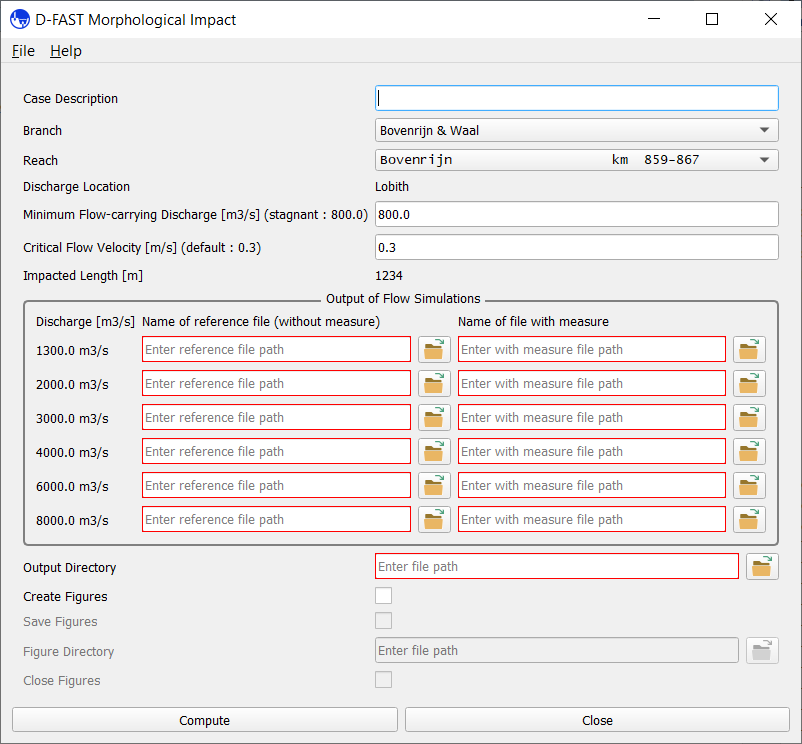
\includegraphics[width=12cm]{figures/main_dialog.png}
\caption{GUI after opening without configuration file}
\label{fig:test1.png}
\end{figure}
\end{enumerate}

\subsection{Test 2: save default configuration file}
\begin{enumerate}
\item Start from Test 1.
\item Select \menu{File} \textrightarrow \menu{Save}, and save the configuration file in the work folder as \file{test2}.
\item Verify that a file \file{test2.cfg} has been created and that the content matches

\verbfilenobox[\scriptsize]{figures/test2.cfg}
\end{enumerate}

\subsection{Test 3: modify settings}
\begin{enumerate}
\item Start from Test 2.
\item Specify "Test 3" as the Case description
\item Select branch "Maas"
\item Verify that the selected reach switches to Grensmaas, that the discharge location switches to Borgharen, and the (rounded) impacted length becomes \SI{0}{\metre}.
\item Select reach "Grave-Lith"
\item Verify that the impacted length becomes \SI{65}{\metre}.
\item Set the minimum flow-carrying discharge to \SI{2100}{\metre\cubed\per\second}
\item Verify that the impacted length reduces to \SI{8}{\metre}, and that the entry boxes for all discharges less or equal to 2100 are greyed-out.
\item Select from the folder \file{tests/c01 - GendtseWaardNevengeul} included in the \dfmi source code repository, the files \file{reference-Q1\_map.nc} and \file{measure-Q1\_map.nc} for the \SI{2500.0}{\metre\cubed\per\second} condition, and \file{reference-Q2\_map.nc} and \file{measure-Q2\_map.nc} for the \SI{3200.0}{\metre\cubed\per\second} condition as shown in \autoref{fig:test3.png}.
\item Verify that the red outline of the edit fields turns grey when valid file names are specified.
\item Select the output directory as \file{d:\textbackslash}.
\item Verify that the red outline of the edit field turns grey to signal that an existing path is specified.
\item Check the create figures box.
\item Verify that the Save and Close figures check boxes are activated when the create figures box is checked.
\item Verify that the dialog matches the following figure
\begin{figure}[H]
\center
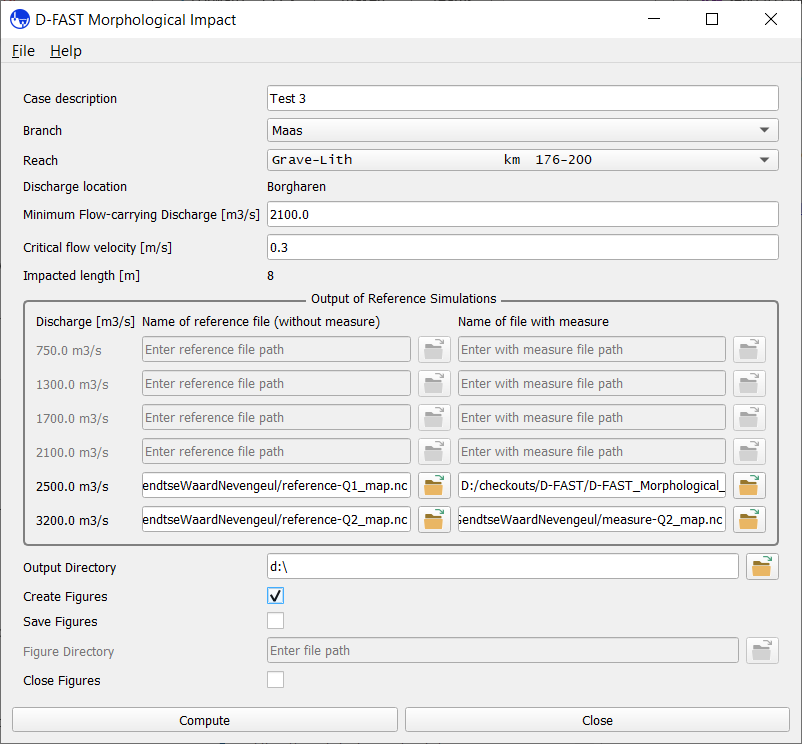
\includegraphics[width=12cm]{figures/test3.png}
\caption{GUI with edits}
\label{fig:test3.png}
\end{figure}
\end{enumerate}

\subsection{Test 4: save modified configuration file}
\begin{enumerate}
\item Start from Test 3.
\item Select \menu{File} \textrightarrow \menu{Save}, and save the configuration file in the work folder as \file{test4.cfg}.
\item Verify that a file \file{test4.cfg} has been created and that the content matches the following listing, but note that the relative paths may differ dependent on the work folder used

\verbfilenobox[\scriptsize]{figures/test4.cfg}
\end{enumerate}

\subsection{Test 5: load default configuration file}
\begin{enumerate}
\item Start from Test 4.
\item Select \menu{File} \textrightarrow \menu{Load}, and select the configuration file \file{test2.cfg}.
\item Verify that the dialog matches \autoref{fig:test1.png}.
\end{enumerate}

\subsection{Test 6: load modified configuration file}
\begin{enumerate}
\item Start from Test 5.
\item Select \menu{File} \textrightarrow \menu{Load}, and select the configuration file "test4.cfg".
\item Verify that the dialog matches \autoref{fig:test3.png}.
\end{enumerate}

\subsection{Test 7: view manual and about Windows}
\begin{enumerate}
\item Start from Test 6.
\item Select \menu{Help} \textrightarrow \menu{Open User Manual} and verify that the user manual is opened.
\item Select \menu{Help} \textrightarrow \menu{Version} and verify that the about box shown matches the image stored as "test7\_about.png" \autoref{fig:manual_system_test_7_about_dfastmi.png} except for the version number (which should match the version being tested) and the copyright year (which should match the year of the latest code update).
\begin{figure}[H]
	\center
	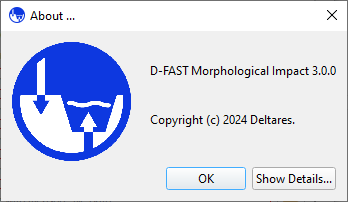
\includegraphics[width=8cm]{figures/manual_system_test_7_about_dfastmi.png}
	\caption{The \dfmi about box showing version and license information.}
	\label{fig:manual_system_test_7_about_dfastmi.png}
\end{figure}
\item Verify that pressing the \button{Show Details...} button reveal a text box stating "This software is distributed under the conditions of the GNU Lesser General Public License Version 2.1; see the LICENSE.md file for details."
\item Close the about box by pressing \button{OK}.
\item Select \menu{Help} \textrightarrow \menu{About Qt} and verify that the about box shown matches the image stored as "test7\_qt.png" \autoref{fig:manual_system_test_7_about_qt.png}.
\begin{figure}[H]
	\center
	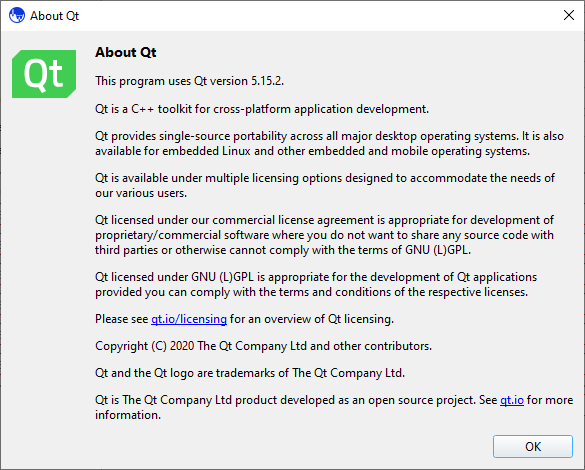
\includegraphics[width=12cm]{figures/manual_system_test_7_about_qt.png}
	\caption{The "About Qt" box.}
	\label{fig:manual_system_test_7_about_qt.png}
\end{figure}
\item Close the "About Qt" box by pressing \button{OK}.
\end{enumerate}

\subsection{Test 8: run \dflowfm analysis}
\begin{enumerate}
\item Start from Test 7.
\item Press the \button{Compute} button.
\item Verify that the analysis completes successfully.
\item The generated figure should correspond to \autoref{fig:report_Figure1.png}.
\item The content of the \file{report.txt} file in the output folder, should be equal to the following \hyperlink{code-report}{listing}.
\item Open the \file{dfastmi\_results.nc} file in QUICKPLOT.
Select the quantity "year-averaged bed level change without dredging" , and plot it using default settings.
See \autoref{fig:manual_system_test_8_quickplot_usage.png} for a snapshot of the steps in QUICKPLOT.
The resulting figure should correspond to \autoref{fig:report_Figure1_QP.png}.
\begin{figure}[H]
\center
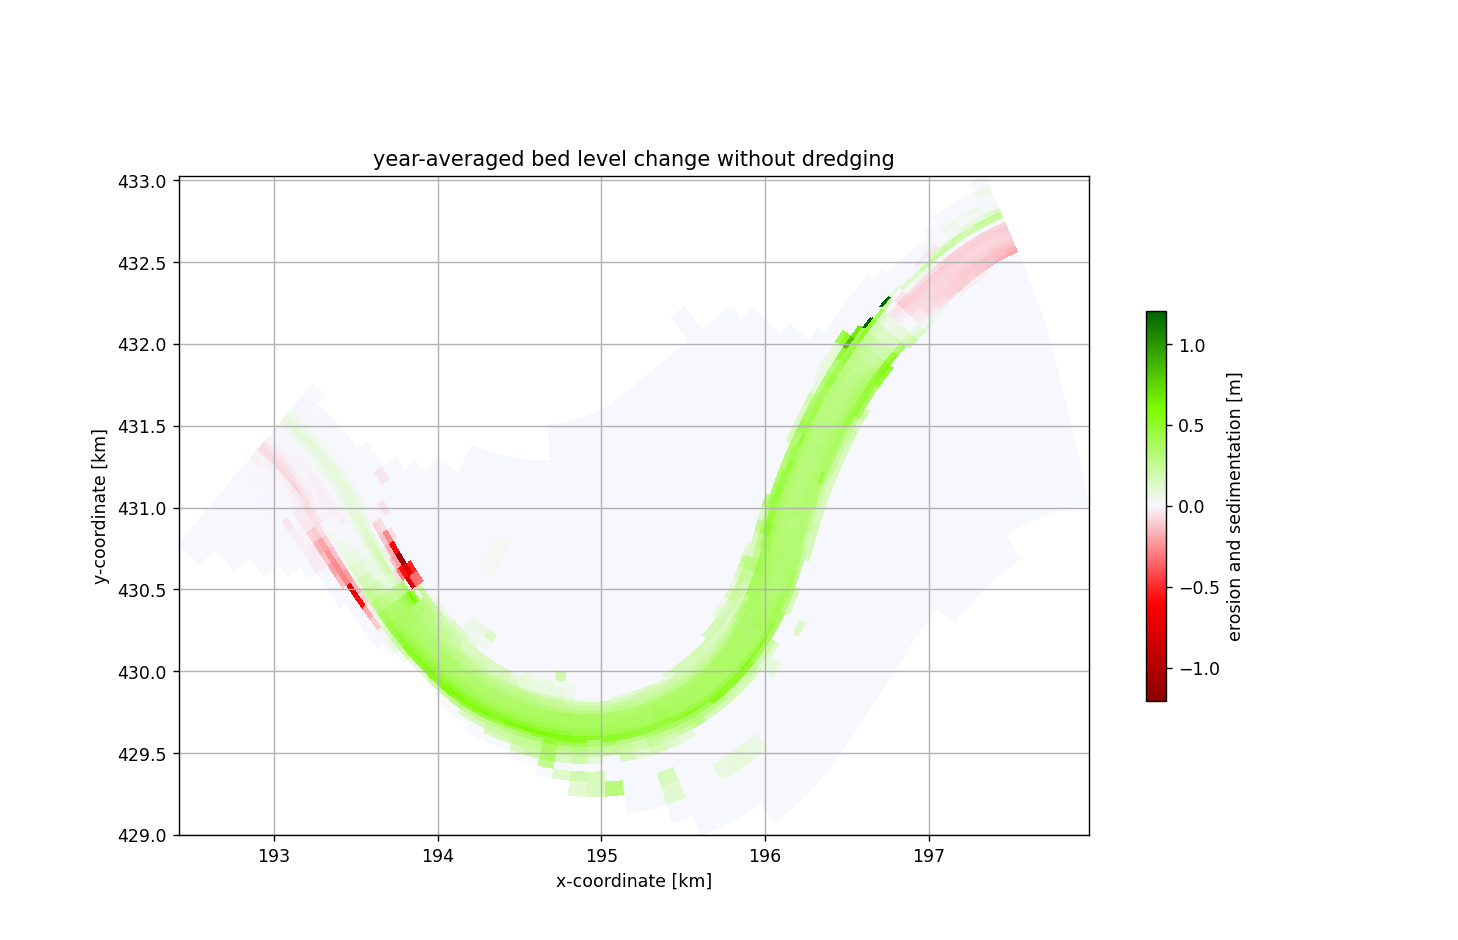
\includegraphics[width=12cm]{figures/report_Figure1.png}
\caption{Analysis results as plotted by \dfmi itself.}
\label{fig:report_Figure1.png}
\end{figure}
\end{enumerate}

\hypertarget{code-report}{\verbfilenobox[\scriptsize]{figures/report.txt}}

\begin{figure}[H]
	\center
	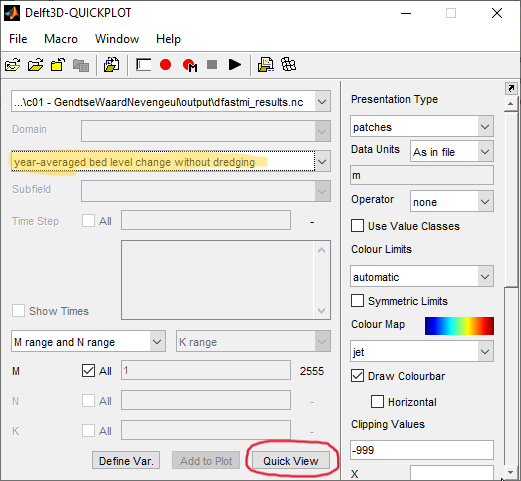
\includegraphics[width=12cm]{figures/manual_system_test_8_quickplot_usage.png}
	\caption{QUICKPLOT settings to create \autoref{fig:report_Figure1_QP.png}.}
	\label{fig:manual_system_test_8_quickplot_usage.png}
\end{figure}

\begin{figure}[H]
\center
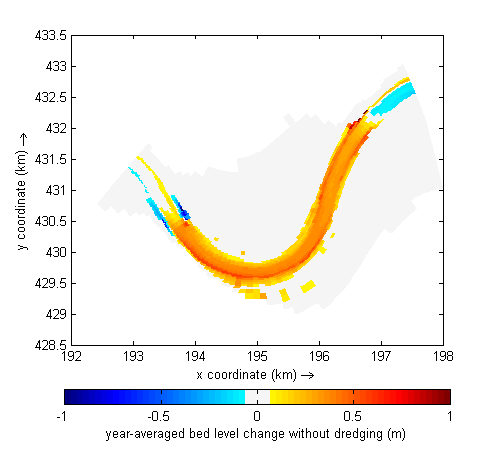
\includegraphics[width=12cm]{figures/report_Figure1_QP.png}
\caption{Analysis results as plotted using QUICKPLOT.}
\label{fig:report_Figure1_QP.png}
\end{figure}

\subsection{Test 9: closing the software}
\begin{enumerate}
\item Start from 8.
\item Close the program by one of the following methods:
\begin{itemize}
\item Select \menu{File} \textrightarrow \menu{Close}.
\item Press the \texttt{x} in the upper-right corner.
\item Press the \button{Close} button.
\end{itemize}
\item Reopen the program and test the other methods.
\item Verify that the program closes without any error using all methods.
\end{enumerate}

%-------------------------------
\chapter{Test Report} \label{Chp:TestReport}

The test plan describes (automated) regression tests, manual tests and the code quality checks.

\section{Manual tests}

This section summarizes the results of the manual testing of the graphical user interface.

\begin{tabular}{ll|l}
Test & Description & Success / Comments \\ \hline
1 & starting blank & OK \\
2 & save default configuration file & OK \\
3 & modify settings & OK \\
4 & save modified configuration file & OK \\
5 & load default configuration file & OK \\
6 & load modified configuration file & OK \\
7 & view manual and about Windows & OK \\
8 & run \dflowfm analysis & OK \\
9 & closing the software & OK \\
\end{tabular}


\section{Automated tests}

Below a brief pytest report of the automated regression testing is included below showing the number of source code lines per file, the number of lines \emph{not} covered by the source code testing phase and the resulting code coverage.
Note that the \keyw{\_\_main\_\_} module code is only executed in the binary testing phase.

\begin{Verbatim}
---------- coverage: platform win32, python 3.9.13-final-0 -----------
Name                                               Stmts   Miss  Cover
----------------------------------------------------------------------
dfastmi\__init__.py                                     4      0   100%
dfastmi\__main__.py                                    50     50     0%
dfastmi\batch\AFileNameRetriever.py                    12      0   100%
dfastmi\batch\AnalyserAndReporterDflowfm.py            16      0   100%
dfastmi\batch\AnalyserAndReporterWaqua.py              12      0   100%
dfastmi\batch\AnalyserDflowfm.py                      215     12    94%
dfastmi\batch\AnalyserWaqua.py                        150      1    99%
dfastmi\batch\AreaDetector.py                         108      0   100%
dfastmi\batch\AreaPlotter.py                           78      0   100%
dfastmi\batch\DFastUtils.py                            49     38    22%
dfastmi\batch\DflowfmReporters.py                      95     33    65%
dfastmi\batch\Distance.py                              54      6    89%
dfastmi\batch\Face.py                                  69      3    96%
dfastmi\batch\FileNameRetriever.py                     25      0   100%
dfastmi\batch\FileNameRetrieverFactory.py              22      0   100%
dfastmi\batch\FileNameRetrieverLegacy.py               14      0   100%
dfastmi\batch\FileNameRetrieverUnsupported.py           7      0   100%
dfastmi\batch\OutputDataDflowfm.py                     60      0   100%
dfastmi\batch\OutputDataWaqua.py                        9      0   100%
dfastmi\batch\PlotOptions.py                           81      3    96%
dfastmi\batch\Projection.py                            56     16    71%
dfastmi\batch\ReporterDflowfm.py                      108      0   100%
dfastmi\batch\ReporterWaqua.py                         20      0   100%
dfastmi\batch\SedimentationData.py                     11      0   100%
dfastmi\batch\SedimentationVolume.py                  125      3    98%
dfastmi\batch\XykmData.py                             115      1    99%
dfastmi\batch\XyzFileWriter.py                         15      0   100%
dfastmi\batch\core.py                                 211     12    94%
dfastmi\batch\plotting.py                             121     50    59%
dfastmi\cli.py                                        235     70    70%
dfastmi\cmd.py                                         28     28     0%
dfastmi\config\AConfigurationChecker.py                37      3    92%
dfastmi\config\AConfigurationInitializerBase.py        76      0   100%
dfastmi\config\ConfigFileOperations.py                127     16    87%
dfastmi\config\ConfigurationChecker.py                 59     11    81%
dfastmi\config\ConfigurationCheckerFactory.py          21      0   100%
dfastmi\config\ConfigurationCheckerLegacy.py           55      4    93%
dfastmi\config\ConfigurationCheckerValidator.py        13      0   100%
dfastmi\config\ConfigurationInitializer.py            104      5    95%
dfastmi\config\ConfigurationInitializerFactory.py      24      1    96%
dfastmi\config\ConfigurationInitializerLegacy.py       52      0   100%
dfastmi\gui\dialog_model.py                           140      1    99%
dfastmi\gui\dialog_utils.py                            56      0   100%
dfastmi\gui\dialog_view.py                            456     34    93%
dfastmi\gui\dialog_view_model.py                      162      4    98%
dfastmi\gui\qt_tools.py                                20      6    70%
dfastmi\io\AReach.py                                   20      0   100%
dfastmi\io\ApplicationSettingsHelper.py                43      0   100%
dfastmi\io\Branch.py                                   33      1    97%
dfastmi\io\CelerObject.py                              53      1    98%
dfastmi\io\ConfigBooleans.py                            2      0   100%
dfastmi\io\DFastAnalysisConfigFileParser.py            34      0   100%
dfastmi\io\DFastRiverConfigFileParser.py               87      0   100%
dfastmi\io\DataTextFileOperations.py                   65      1    98%
dfastmi\io\IBranch.py                                  16      0   100%
dfastmi\io\IReach.py                                   13      0   100%
dfastmi\io\ObservableList.py                           25      0   100%
dfastmi\io\Reach.py                                    48      0   100%
dfastmi\io\ReachLegacy.py                              11      0   100%
dfastmi\io\RiversObject.py                            120      2    98%
dfastmi\io\map_file.py                                138      3    98%
dfastmi\kernel\BedLevelCalculator.py                   60      0   100%
dfastmi\kernel\core.py                                 30      0   100%
dfastmi\kernel\legacy.py                               55      0   100%
dfastmi\kernel\typehints.py                             6      0   100%
dfastmi\resources.py                                    4      0   100%
-----------------------------------------------------------------------
TOTAL                                                4440    419    91%

====================== 455 passed, 33 warnings in 39.77s ======================
\end{Verbatim}

\section{Code check}
The quality of the \dfastmi source code and the code coverage is tracked by \href{https://sonarcloud.io/project/overview?id=Deltares_D-FAST_Morphological_Impact}{SonarCloud} and \href{https://sigrid-says.com/deltares/dfast-mi/-/overview}{Sigrid}.

\subsection{SonarCloud reports}
During the development of D-FAST MI 3.0.0, the number of code lines has doubled.
There is no duplication in the code anymore, see \autoref{fig:code_duplication}.
At the time of the first upload about 40\% of the code was covered by a limited set of about 65 tests.
The code coverage was still relatively high due to a few system tests that touched a lot of lines of code.
Since that time, the code coverage has increased to 90\% whereas at the same time the number of code lines has increased from about 2700 to almost 4400.
See \autoref{fig:code_coverage}.
During the same period the number of code issues detected by SonarCloud has decreased from 240 to 65.
Out of the remaining 65 issues, 15 are considered high severity, 20 medium severity and 30 low severity.
The 15 most critical issues are related to code complexity that is slightly too high, and \keyw{try-except} constructs that don't filter the exceptions that they catch.
See \autoref{fig:code_issues}.

\begin{figure}
\center
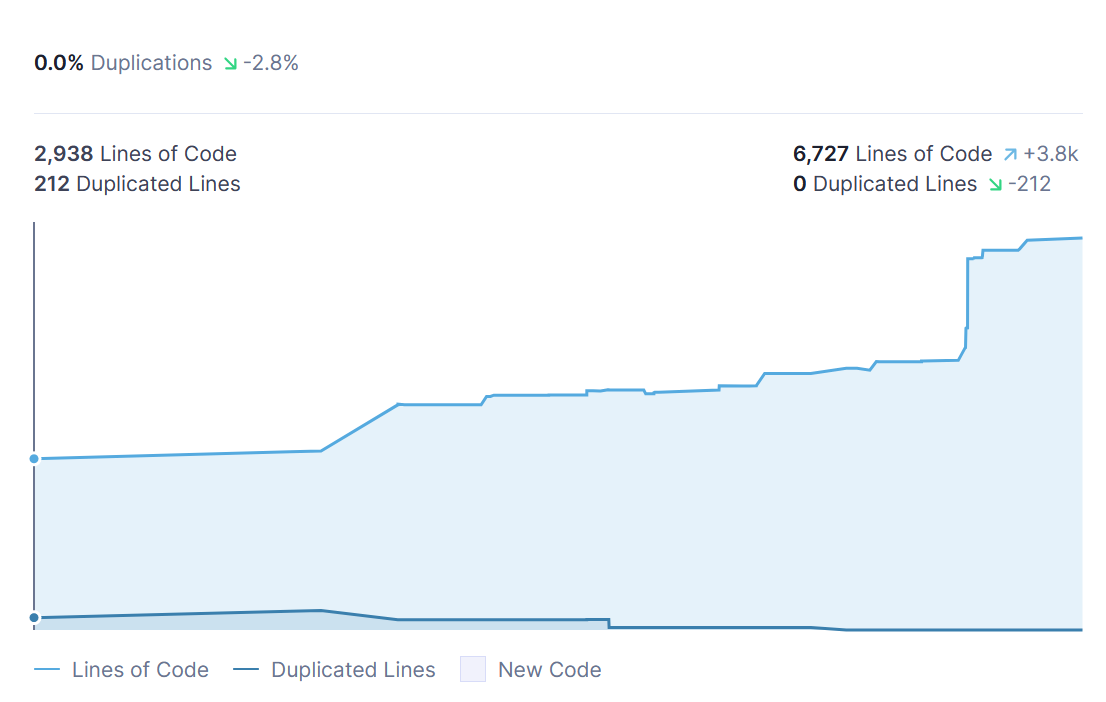
\includegraphics[width=10cm]{figures/code_duplication.png}
\caption{Code duplication}
\label{fig:code_duplication}
\end{figure}

\begin{figure}
\center
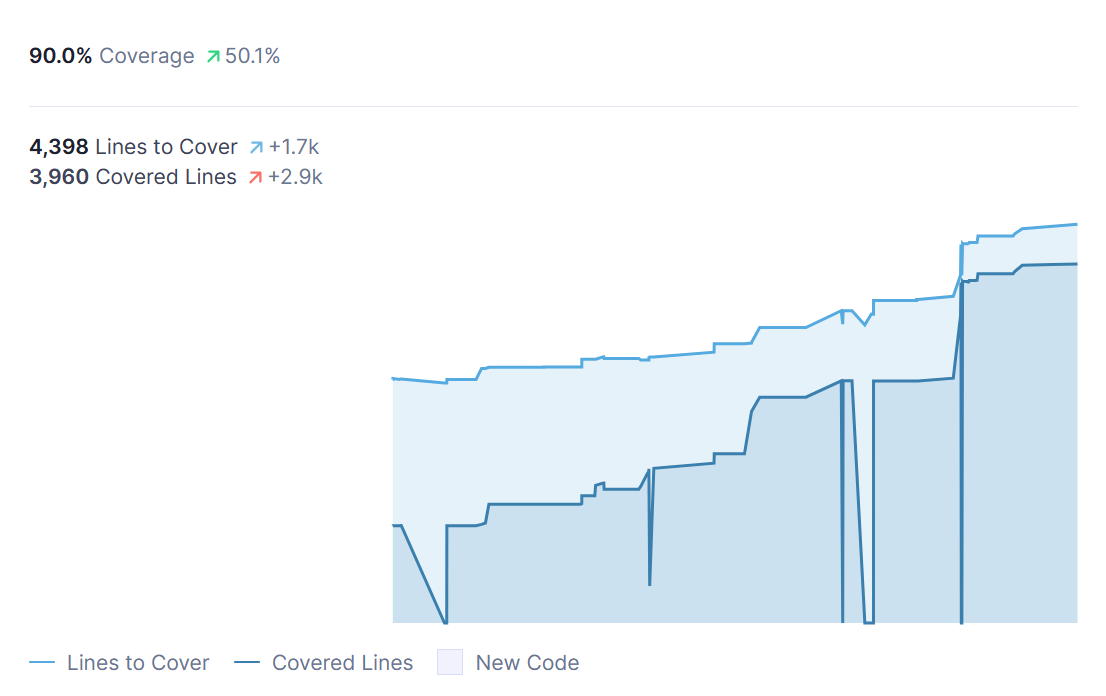
\includegraphics[width=10cm]{figures/code_coverage.png}
\caption{Code coverage}
\label{fig:code_coverage}
\end{figure}

\begin{figure}
\center
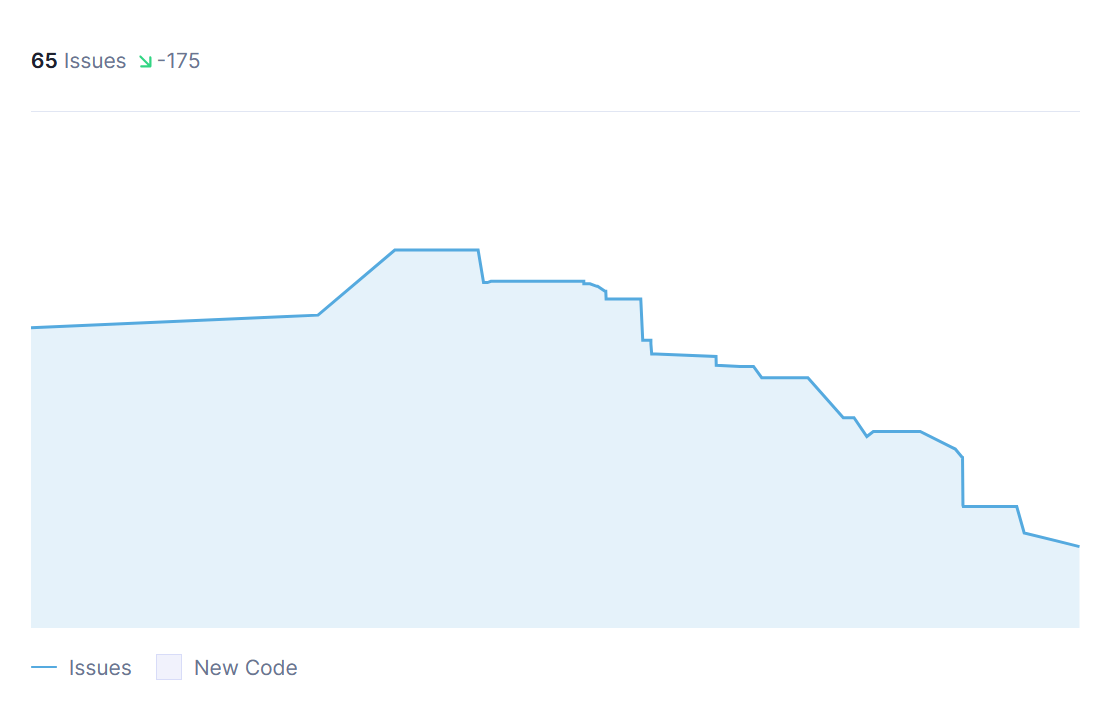
\includegraphics[width=10cm]{figures/code_issues.png}
\caption{Number of code issues flagged by SonarCloud}
\label{fig:code_issues}
\end{figure}

\subsection{Sigrid report}
The overall maintainability is scored at 3.6, with an architecture score of 3.4.
The total amount of code represents 11 person months (to develop).
The number of lines of code for testing is almost the same as the number of lines of code for the program itself (test/code ration = 92 \%).
The code depends on 60 open source libraries of which 5 (cftime, click-plugins, intel-openmp, mkl, tbb) are marked as high risk since the version used is more than 1 year old.
There is 1 critical security issue.
This is related to the opening the user manual by starting a shell process; someone might exploit this by starting some other process.

\begin{figure}
\center
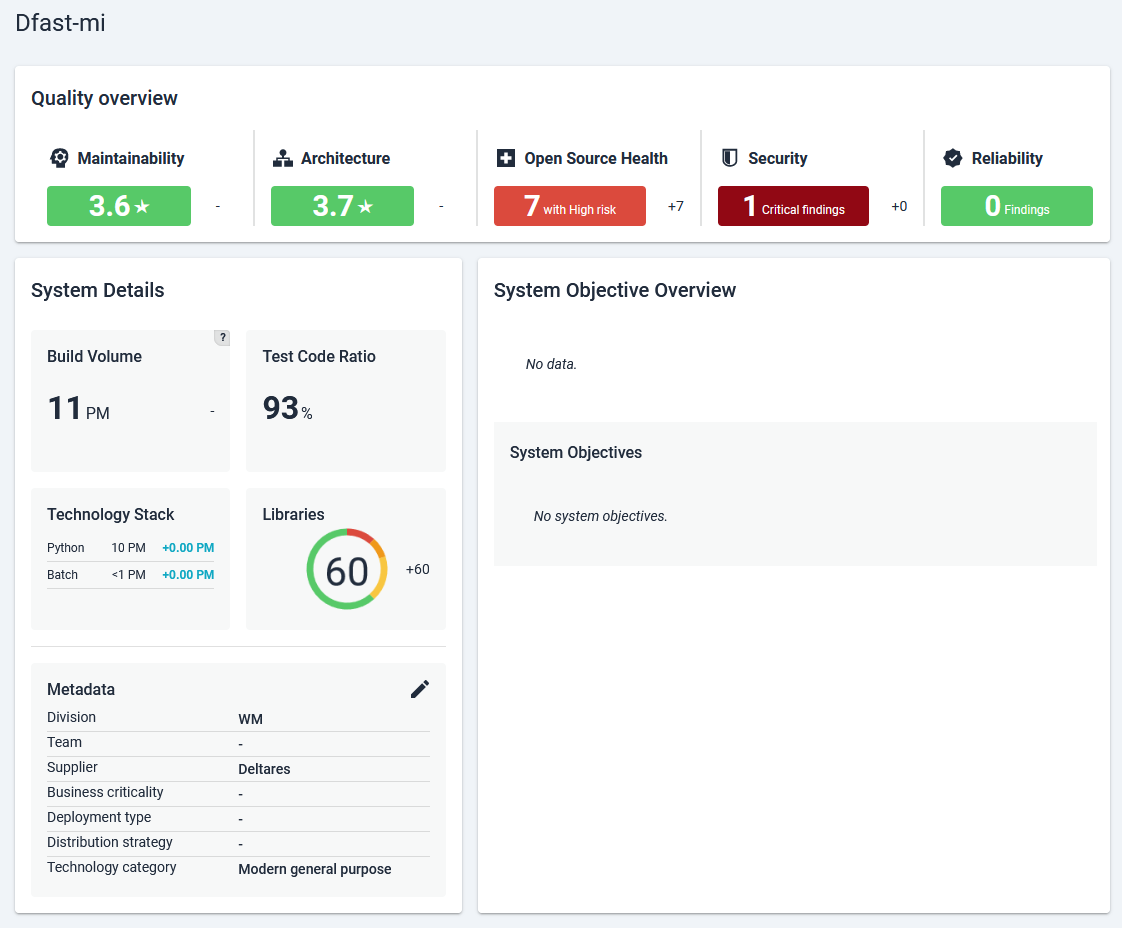
\includegraphics[width=\textwidth]{figures/sigrid.png}
\caption{Sigrid Overview}
\label{fig:sigrid_overview}
\end{figure}

\begin{figure}
\center
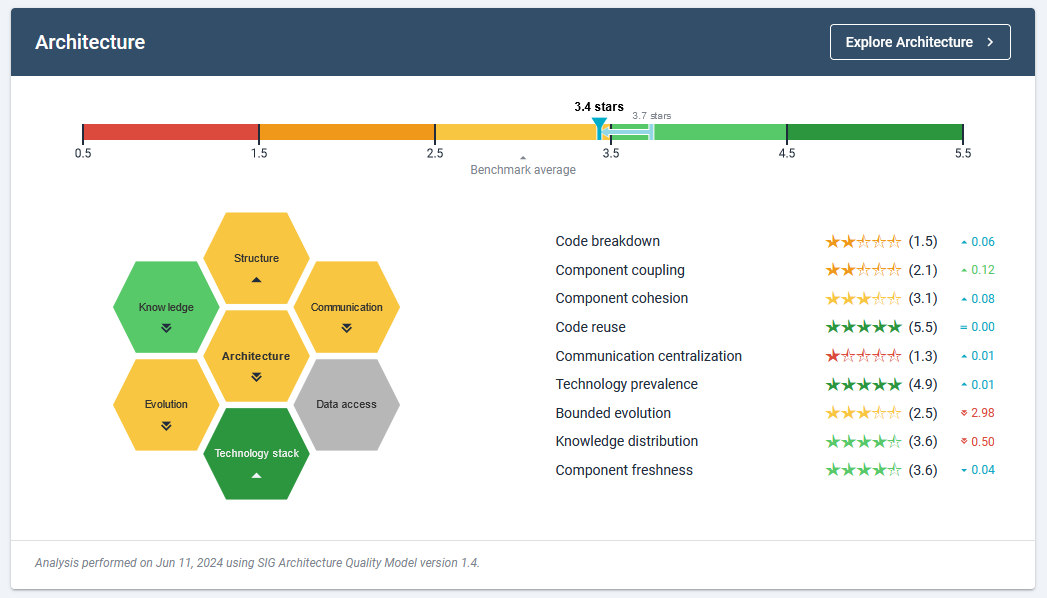
\includegraphics[width=\textwidth]{figures/sigrid-architecture.png}
\caption{Sigrid summary of architecture aspects}
\label{fig:sigrid_architecture_overview}
\end{figure}

\begin{figure}
\center
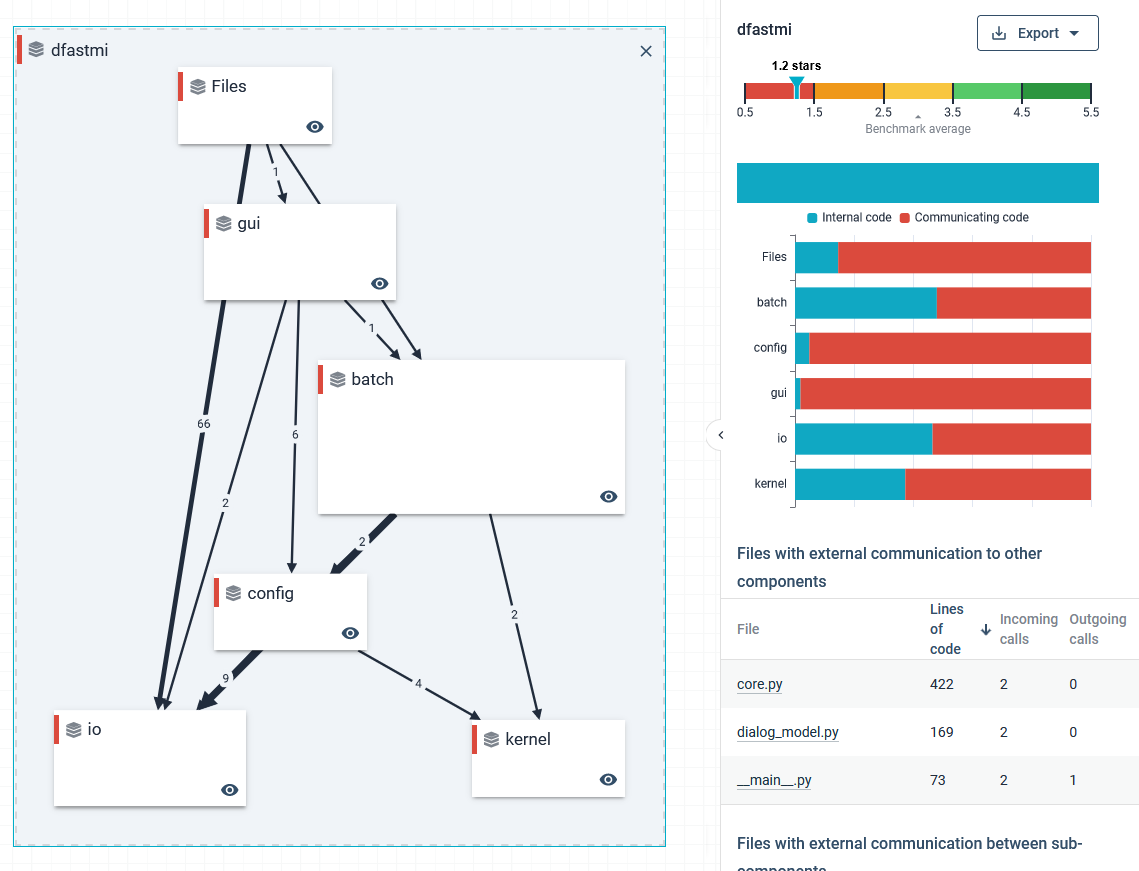
\includegraphics[width=\textwidth]{figures/sigrid-arch-communication.png}
\caption{Sigrid evaluation of communication centralization}
\label{fig:sigrid_architecture_comm}
\end{figure}
